\documentclass[tikz,border=5pt]{standalone}
\usepackage{amsmath,amssymb,mathtools}
\usepackage{braket}
\usepackage{xcolor}
\usepackage{tikz}
\usetikzlibrary{arrows.meta,decorations.pathmorphing,decorations.pathreplacing,calc,positioning}

\definecolor{cobalt}{HTML}{2b4c7e}
\definecolor{boxblue}{HTML}{eef3fa}
\definecolor{boxgold}{HTML}{fbf3e3}
\definecolor{boxred}{HTML}{fbecec}
\definecolor{boxgreen}{HTML}{eaf6f0}
\definecolor{ruleblue}{HTML}{2b6cb0}
\definecolor{rulegold}{HTML}{b7791f}
\definecolor{rulered}{HTML}{c0392b}
\definecolor{rulegreen}{HTML}{1f8a5f}

\newcommand{\HH}{\mathcal{H}}
\newcommand{\M}{\mathcal{M}}
\newcommand{\tr}{\operatorname{tr}}
\newcommand{\Tr}{\operatorname{Tr}}
\newcommand{\ii}{\mathrm{i}}
\begin{document}
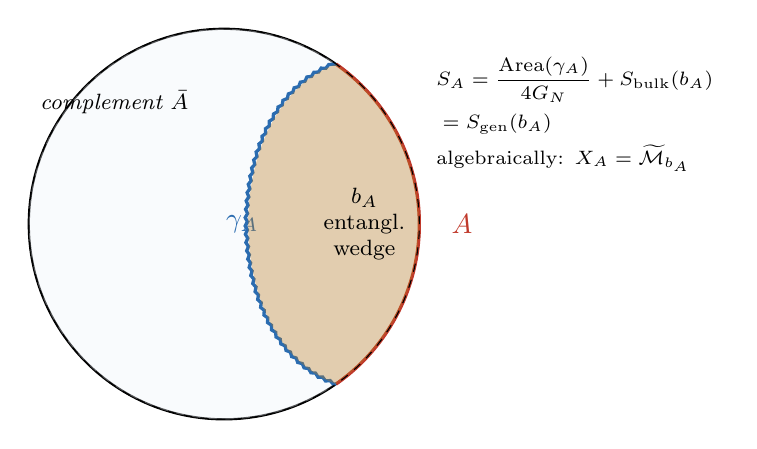
\begin{tikzpicture}[scale=1.55, >=Latex]
  % global AdS constant-time slice as a disk
  \draw[thick] (0,0) circle (1.6);
  \fill[boxblue, opacity=0.35] (0,0) circle (1.6);
  % boundary region A: arc from -50 to 50 deg
  \draw[very thick, rulered] (1.6*cos{-55}, 1.6*sin{-55}) arc (-55:55:1.6);
  \node[rulered] at (1.95,0) {$A$};
  % RT surface: geodesic chord connecting endpoints of A (approx as circular arc bulging left, using a simple chord for schematic)
  \draw[very thick, ruleblue, decorate, decoration={snake, amplitude=0.4pt, segment length=3pt}]
     (1.6*cos{-55}, 1.6*sin{-55}) to[out=160,in=-160] (1.6*cos{55}, 1.6*sin{55});
  \node[ruleblue] at (0.15,0) {$\gamma_A$};
  % shade entanglement wedge region b_A between A and gamma_A
  \begin{scope}
    \clip (1.6*cos{-55}, 1.6*sin{-55}) arc (-55:55:1.6) -- (1.6*cos{55}, 1.6*sin{55}) to[out=-160,in=160] (1.6*cos{-55}, 1.6*sin{-55}) -- cycle;
    \fill[rulegold, opacity=0.35] (0,0) circle (1.6);
  \end{scope}
  \node[font=\footnotesize, align=center] at (1.15,0) {$b_A$\\ entangl.\\ wedge};
  \node[font=\footnotesize] at (-0.9,1.0) {\it complement $\bar A$};
  \draw[dashed] (0,0) circle (1.6);
  % small legend arrow
  \node[font=\scriptsize, align=left, text width=3.6cm] at (2.9,0.9)
   {$S_A = \dfrac{\mathrm{Area}(\gamma_A)}{4G_N}+S_{\rm bulk}(b_A)$\\[3pt]
    $\;=S_{\rm gen}(b_A)$\\[3pt]
    algebraically: $X_A=\widetilde\M_{b_A}$};
\end{tikzpicture}

\end{document}
